% 
% Lecture Template for ME3023 -  Measurements in Mechanical Systems - Tennessee Technological University
%
% Spring 2020 - Summer 2020
% Tristan Hill, May 07, 2020 - June 12, 2020
% Module 5 - Strain Applications
% Topic 1 - Beam Models
%

\documentclass{beamer}                         % for presentation (has nav buttons at bottom)
%\documentclass[handout]{beamer}  % for handout 
\usepackage{beamerthemesplit}
\usepackage{amsmath}
\usepackage{listings}
\usepackage{multicol}
\usepackage{framed}

\beamertemplateballitem

% custom colors
\definecolor{TTUpurple}{rgb}{0.3098, 0.1607, 0.5176} % TTU Purple (primary)
\definecolor{TTUgold}{rgb}{1.0000, 0.8666, 0.0000} % TTU Gold (primary) 
\definecolor{mygray}{rgb}{.6, .6, .6}
\definecolor{mypurple}{rgb}{0.6,0.1961,0.8}
\definecolor{mybrown}{rgb}{0.5451,0.2706,0.0745}
\definecolor{mygreen}{rgb}{0, .39, 0}
\definecolor{mypink}{rgb}{0.9960, 0, 0.9960}

% color commands
\newcommand{\R}{\color{red}}
\newcommand{\B}{\color{blue}}
\newcommand{\BR}{\color{mybrown}}
\newcommand{\K}{\color{black}}
\newcommand{\G}{\color{mygreen}}
\newcommand{\PR}{\color{mypurple}}
\newcommand{\PN}{\color{mypink}}
\newcommand{\OR}{\color{TTU}}
\newcommand{\GD}{\color{TTUgold}}


\setbeamercolor{palette primary}{bg=TTUpurple,fg=TTUgold}
\setbeamercolor{palette secondary}{bg=black,fg=TTUgold}
\setbeamercolor{palette tertiary}{bg=black,fg=TTUpurple}
\setbeamercolor{palette quaternary}{bg=TTUgold,fg=black}
\setbeamercolor{structure}{fg=TTUpurple} % itemize, enumerate, etc
\setbeamercolor{section in toc}{fg=TTUpurple} % TOC sections

%\usefonttheme{professionalfonts}

\newcommand{\Lagr}{\mathcal{L}} % lagrangian

\newcommand{\hspcu}{\underline{\hspace{20mm}}} % large horizontal space w underline
\newcommand{\vspccc}{\vspace{6mm}\\} % large vertical space
\newcommand{\vspcc}{\vspace{4mm}\\}   % medium vertical space
\newcommand{\vspc}{\vspace{2mm}\\}     % small vertical space

\newcommand{\hspcccc}{\hspace{10mm}} % large horizontal space
\newcommand{\hspccc}{\hspace{6mm}} % large horizontal space
\newcommand{\hspcc}{\hspace{4mm}}   % medium horizontal space
\newcommand{\hspc}{\hspace{2mm}}     % small horizontal space

\newcommand{\eqscl}{0.9}     % small horizontal space


\author{ME3023 - Measurements in Mechanical Systems} % original formatting from Mike Renfro, September 21, 2004

\newcommand{\MNUM}{5\hspace{2mm}} % Module number
\newcommand{\TNUM}{1\hspace{2mm}} % Topic number 
\newcommand{\moduletitle}{Strain Applications}
\newcommand{\topictitle}{Beam Models} 

\newcommand{\sectiontitleI}{Euler–Bernoulli Beam Theory}
\newcommand{\sectiontitleII}{Force-Deflection Model}
\newcommand{\sectiontitleIII}{Cantilevered Beam}
\newcommand{\sectiontitleIV}{Deflection and Strain}

% custom box
\newsavebox{\mybox}

\title{Module \MNUM - \moduletitle}

\date{Mechanical Engineering\vspc Tennessee Technological University}

\begin{document}

\lstset{language=MATLAB,basicstyle=\ttfamily\small,showstringspaces=false}

\frame{\titlepage \center\begin{framed}\Large \textbf{Topic \TNUM - \topictitle}\end{framed} \vspace{5mm}}

% Section 0: Outline
\frame{

\large \textbf{Topic \TNUM - \topictitle} \vspace{3mm}\\

\begin{multicols}{2}
\begin{itemize}

	\item \sectiontitleI    \vspc % Section I
	\item \sectiontitleII 	\vspc % Section II
	\item \sectiontitleIII 	\vspc %Section III
	\item \sectiontitleIV 	\vspc %Section IV

\end{itemize}

\includegraphics[scale=0.28]{leonhard_euler.jpg}
\includegraphics[scale=1.7]{daniel_bernoulli.jpg}

\end{multicols}

}

% Section I:
\section{\sectiontitleI}

% Section I - Frame I:
\frame{
\frametitle{\sectiontitleI}
\small

Euler–Bernoulli beam theory (also known as engineer's beam theory or classical beam theory)[1] is a simplification of the linear theory of elasticity which provides a means of calculating the load-carrying and deflection characteristics of beams. It covers the case for small deflections of a beam that are subjected to lateral loads only. 

{\tiny Text: \href{https://en.wikipedia.org/wiki/Euler\%E2\%80\%93Bernoulli_beam_theory}{Wikipedia}}
}

% Section I - Frame II:
\frame{
\frametitle{\sectiontitleI}
\small

It is thus a special case of Timoshenko beam theory. It was first enunciated circa 1750,[2] but was not applied on a large scale until the development of the Eiffel Tower and the Ferris wheel in the late 19th century. Following these successful demonstrations, it quickly became a cornerstone of engineering and an enabler of the Second Industrial Revolution.\vspc

Additional mathematical models have been developed such as plate theory, but the simplicity of beam theory makes it an important tool in the sciences, especially structural and mechanical engineering. 

{\tiny Text: \href{https://en.wikipedia.org/wiki/Euler\%E2\%80\%93Bernoulli_beam_theory}{Wikipedia}}
}


% Section II:
\section{\sectiontitleII}

% Section II - Frame I:
\frame{
\frametitle{\sectiontitleII}

\begin{multicols}{2}
	\includegraphics[scale=.4]{diving_board_cut.png}
	\small
	These stiffness equations come from the beam deflection equations you have and will study.\vspc 
	You can see them \href{https://mechanicalc.com/reference/beam-deflection-tables}{{\B here}} or look in your copy of Shigleys, and here is a good section on beam analysis \href{https://mechanicalc.com/reference/beam-analysis}{\B analysis}.


	\includegraphics[scale=.2]{types_of_springs.png}
\end{multicols}



}

% Section II - Frame II:
\frame{
\frametitle{\sectiontitleII}

The beam equations relate internal moment and shear as well as deflection along the length of the beam to the given beam geometry and loading.  

\begin{multicols}{2}

\includegraphics[scale=.50]{cantelever_deflection.png}

\vspace{10mm}
\hspccc\scalebox{1}{$\delta(x)=-\frac{Fx^2}{6EI}(3L-x)$} \vspc
\hspccc\scalebox{1}{$\delta_{max}=\delta|_{x=L}=-\frac{FL^3}{3EI}$} \vspccc
\hspccc\scalebox{1}{$\theta(x)=-\frac{Fx}{2EI}(2L-x)$} \vspc
\hspccc\scalebox{1}{$\theta_{max}=\theta|_{x=L}=-\frac{FL^2}{2EI}$}

\end{multicols}

}


% Section III:
\section{\sectiontitleIII}

% Section III - Frame I:
\frame{
\frametitle{\sectiontitleIII}
\small

The shear and moment are both given as a function of x, the direction along the beam. 

\begin{multicols}{2}

\includegraphics[scale=.5]{cantelever_beam.png}

\scalebox{1}{$M(x)=-F(L-x)$}\vspcc
\scalebox{1}{$M_max=M|_{x=0}=-FL$}

\end{multicols}


}

% Section III - Frame II:
\frame{
\frametitle{\sectiontitleIII}
\small

The internal stress is given as a function of y, the distance from the neutral axis. \vspccc

\begin{multicols}{2}

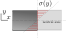
\includegraphics[scale=.75]{internal_stress.png}

\scalebox{1}{$\sigma=\frac{Mc}{I}$}\vspc

\end{multicols}

\vspace{20mm}
{\tiny Text: Theory and Design of Mechanical Measurements}
}

%% Section IV:
\section{\sectiontitleIV}

% Section IV - Frame I:
\frame{
\frametitle{\sectiontitleIV}
\small
Now, with the beam equations you can relate measured strain at a known location to deflection at the end of the beam.These equations are available for many different beam types and loading conditions. {\tiny \href{https://mechanicalc.com/reference/beam-deflection-tables}{{\B Beam Eq's}}}  \vspc

\includegraphics[scale=.4]{axial_gaged_beam.png}


}
	
\end{document}





